\documentclass[11pt,a4paper]{article}

\usepackage[margin=1in]{geometry}
\usepackage{titlesec}
\usepackage{enumitem}
\usepackage{hyperref}
\usepackage{parskip}
\usepackage{graphicx}
\usepackage{float}
\usepackage{booktabs}
\usepackage{amsmath}

\hypersetup{colorlinks=true, linkcolor=blue, urlcolor=blue}

\titleformat{\section}{\large\bfseries}{\thesection}{0.5em}{}
\titleformat{\subsection}{\normalsize\bfseries}{\thesubsection}{0.5em}{}
\setlist{leftmargin=1.4em, topsep=2pt, itemsep=2pt}

\title{\vspace{-1.5cm}\textbf{PKCERT AI \& Software Development Internship \\ Task 16: End-to-End Machine Learning Pipeline Project}}
\author{Abdullah Amir}
\date{AI and Software Development \\ 23 July 2026}

\begin{document}

\maketitle
\vspace{-0.8cm}

This report covers the theory and the results. The full code, outputs and plots live in
the notebook \texttt{house\_price\_pipeline.ipynb}. The dataset is \textbf{Ames Housing}
(De Cock, 2011): 1,460 residential sales in Ames, Iowa, 79 raw features, not used in any
earlier task. This is the capstone task, and it is treated as one: a single pipeline
carries the data from raw CSV to a documented, evaluated model, applying preprocessing,
feature engineering and model comparison together rather than as separate exercises.

% ----------------------------------------------------------------
\section*{Part A: Dataset Selection \& Data Preparation}

\textbf{What the features are.} Each row is one house sale: a mix of 37 numeric
measurements (areas, room counts, year built, etc.) and 43 categorical quality/type
ratings (\texttt{OverallQual}, \texttt{KitchenQual}, \texttt{Neighborhood}, and so on).
The target, \texttt{SalePrice}, is right-skewed (skew 1.88), so the model is trained on
$\log(1 + \text{SalePrice})$, which is close to symmetric (skew 0.12); every error metric
reported below is converted back to dollars for interpretability.

\begin{figure}[H]
    \centering
    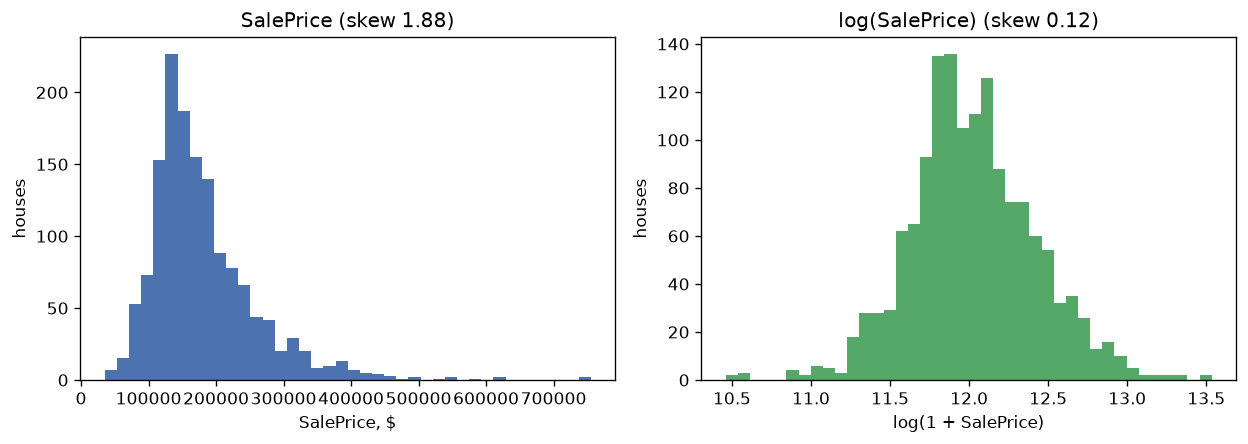
\includegraphics[width=0.95\textwidth]{figures/01_target_distribution.png}
    \caption{SalePrice before and after the log transform.}
\end{figure}

\textbf{Outliers, checked individually rather than filtered by one threshold.} The
dataset's own author documents two specific outliers. The obvious shortcut is to drop
every house above some \texttt{GrLivArea} cutoff, but two of the four largest houses in
this data are simply large, expensive houses, not outliers -- dropping them would throw
away real signal for no reason.

\begin{table}[H]
\centering
\begin{tabular}{lrrl}
\toprule
\textbf{Index} & \textbf{GrLivArea} & \textbf{SalePrice} & \textbf{Verdict} \\
\midrule
1298 & 5,642 & \$160,000 & dropped -- outlier \\
523  & 4,676 & \$184,750 & dropped -- outlier \\
1182 & 4,476 & \$745,000 & kept -- genuinely large and expensive \\
691  & 4,316 & \$755,000 & kept -- genuinely large and expensive \\
\bottomrule
\end{tabular}
\caption{Only 2 of the 4 largest houses are genuine outliers.}
\end{table}

\textbf{Missing values: most of them do not mean ``missing''.} In this dataset's data
dictionary, \texttt{NaN} in a quality/type column almost always means the feature simply
does not exist on that house -- \texttt{PoolQC = NaN} means \emph{no pool}, not
\emph{unknown pool quality}. Treating every \texttt{NaN} as something to statistically
impute would be a real mistake; those columns are filled with an explicit
\texttt{"None"} / \texttt{0} instead, and true imputation is reserved for the columns
that are genuinely incomplete: \texttt{LotFrontage} (259 rows, filled with the
\emph{neighbourhood} median, since street frontage tracks a neighbourhood's typical lot
shape far better than one dataset-wide number) and \texttt{Electrical} (1 row, mode).

\begin{figure}[H]
    \centering
    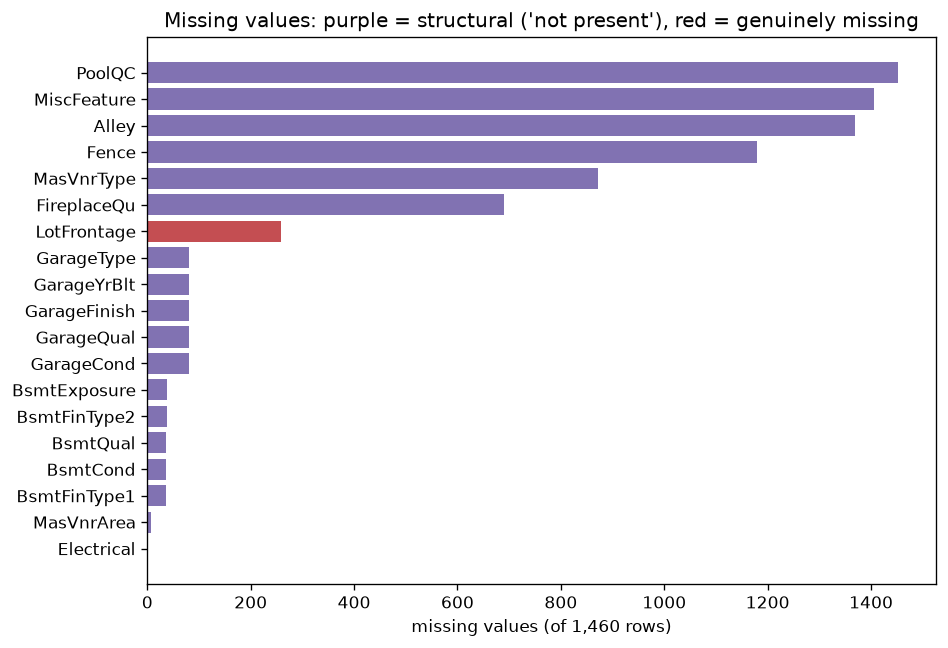
\includegraphics[width=0.72\textwidth]{figures/02_missing_values.png}
    \caption{19 columns have missing values; all but one are structural, not genuine gaps.}
\end{figure}

\textbf{Feature engineering.} Eight features built from domain knowledge of how houses
are actually priced: \texttt{TotalSF} (basement + 1st + 2nd floor area),
\texttt{HouseAge} and \texttt{RemodAge} (years since built / remodelled, relative to
sale year), \texttt{TotalBath} (a single weighted bathroom count), and four presence
flags (\texttt{HasPool}, \texttt{HasGarage}, \texttt{HasFireplace}, \texttt{Has2ndFloor}).

\begin{figure}[H]
    \centering
    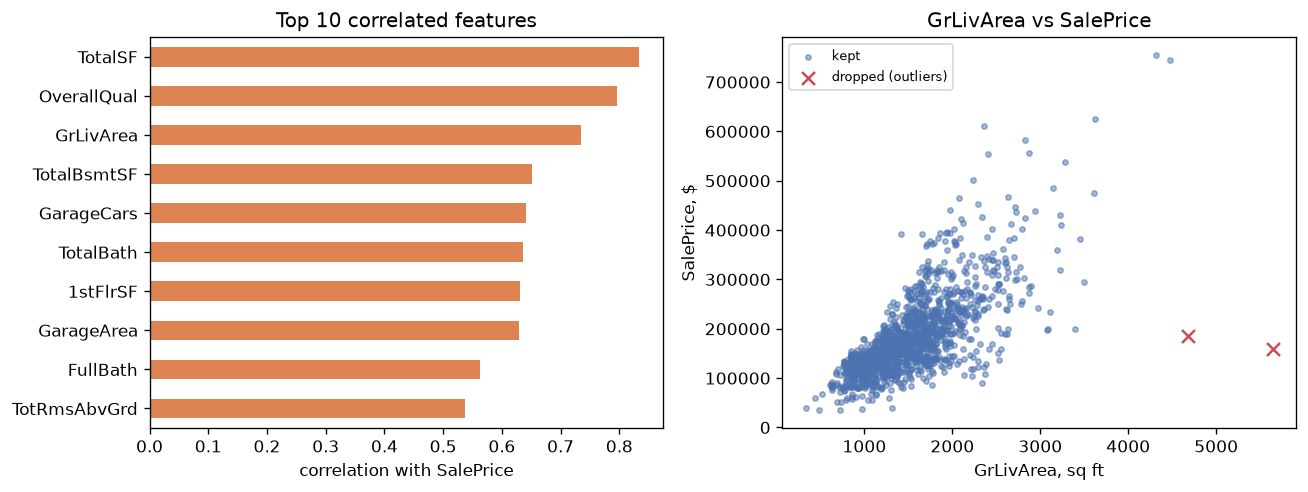
\includegraphics[width=0.95\textwidth]{figures/03_correlations_outliers.png}
    \caption{Left: top 10 features correlated with SalePrice -- the engineered
    \texttt{TotalSF} leads. Right: the outlier decision, visualised.}
\end{figure}

\textbf{The engineered feature is measurably better, not just convenient.}
\texttt{TotalSF} correlates with \texttt{SalePrice} at \textbf{0.833}, higher than either
raw component it was built from (\texttt{1stFlrSF} 0.632, \texttt{TotalBsmtSF} 0.651) and
higher than \texttt{GrLivArea} alone (0.735) -- a checked reason to keep it, not an
assumption that combining features must help.

\begin{figure}[H]
    \centering
    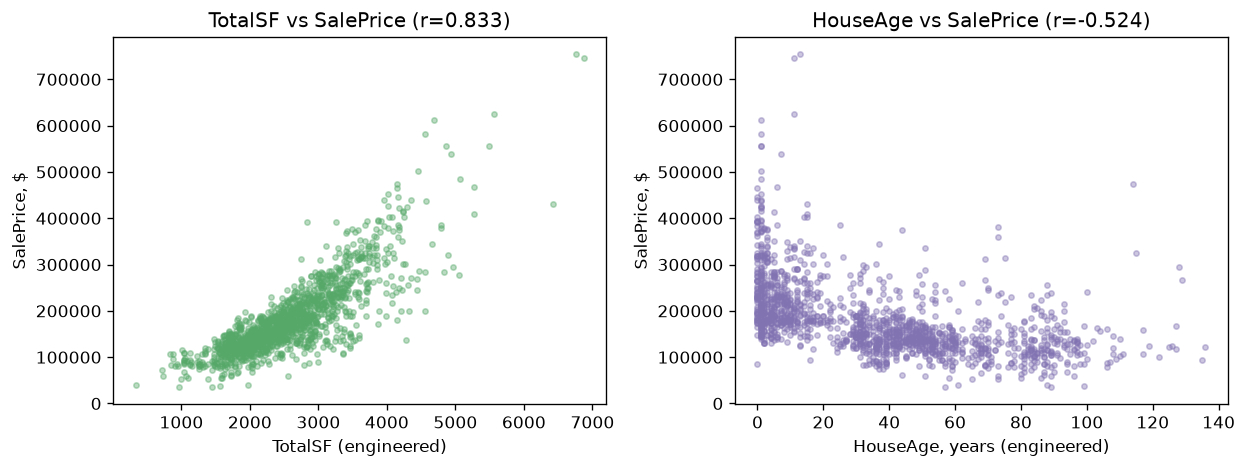
\includegraphics[width=0.95\textwidth]{figures/04_engineered_features.png}
    \caption{The two strongest engineered features against SalePrice.}
\end{figure}

% ----------------------------------------------------------------
\section*{Part B: Model Development}

A single \texttt{ColumnTransformer} handles both feature types: numeric columns are
median-imputed (for any residual gaps) and standard-scaled; categorical columns are
most-frequent-imputed and one-hot encoded, expanding to 87 total features. Two models
share this exact preprocessing inside one \texttt{Pipeline} object each, so the
comparison below isolates the \emph{model}, not the pipeline around it.

\begin{table}[H]
\centering
\begin{tabular}{lrrrrr}
\toprule
\textbf{Model} & \textbf{CV RMSE (log)} & \textbf{CV R\textsuperscript{2}} & \textbf{Test R\textsuperscript{2}} & \textbf{Test RMSE} & \textbf{Test MAE} \\
\midrule
Ridge Regression & \textbf{0.1120 $\pm$ 0.010} & \textbf{0.9191} & \textbf{0.9095} & \textbf{\$20,155} & \textbf{\$14,611} \\
Random Forest & 0.1353 $\pm$ 0.013 & 0.8829 & 0.8764 & \$23,600 & \$16,367 \\
\bottomrule
\end{tabular}
\caption{5-fold cross-validation on the training set, then held-out test metrics.}
\end{table}

\begin{figure}[H]
    \centering
    
\includegraphics[width=0.85\textwidth]{figures/05_model_comparison.png}
    \caption{Ridge ahead of Random Forest in both cross-validation and on the test set.}
\end{figure}

\textbf{Ridge beat Random Forest on every metric}, in cross-validation and on the
held-out test set alike. With 87 features after one-hot encoding and 1,166 training
rows, most of the real signal -- \texttt{OverallQual}, \texttt{TotalSF}, and dozens of
one-hot category indicators -- genuinely does relate to log-price close to linearly,
which plays to Ridge's strength, and its regularisation keeps the wide, sparse
categorical block from overfitting. The Random Forest used here was not
hyperparameter-tuned (400 trees, default depth); Part C returns to this as a stated
limitation rather than a general verdict on tree ensembles.

% ----------------------------------------------------------------
\section*{Part C: Model Evaluation}

\begin{figure}[H]
    \centering
    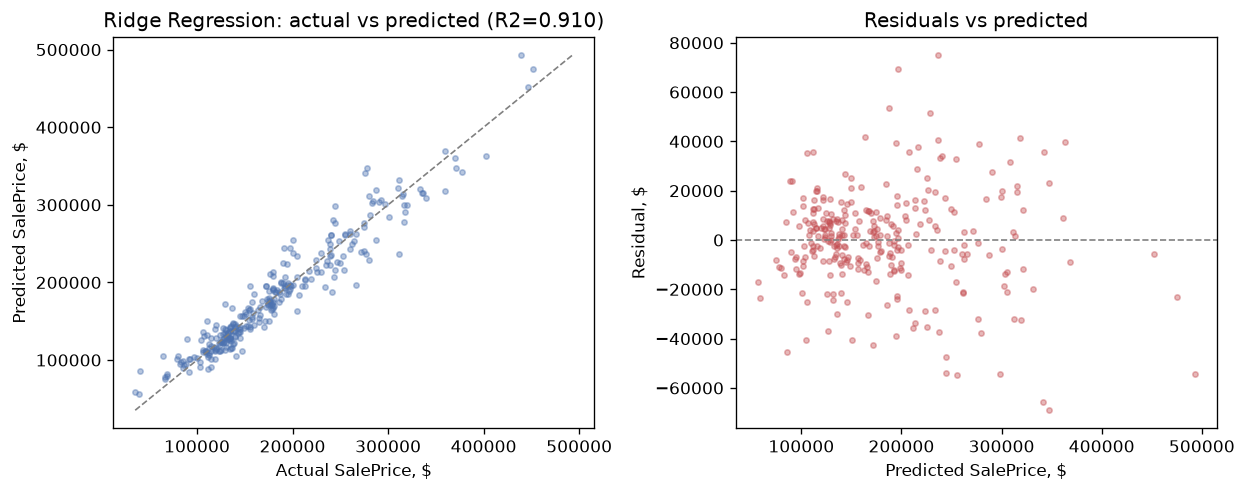
\includegraphics[width=0.95\textwidth]{figures/06_diagnostics.png}
    \caption{Ridge Regression, the chosen model: actual vs predicted, and residuals.}
\end{figure}

\textbf{Reading the diagnostics.} The actual-vs-predicted scatter tracks the diagonal
closely across the bulk of the price range (\$100k--\$300k, where most of the data
sits). The residual plot shows two things worth stating plainly rather than hiding
behind the single R\textsuperscript{2} number: residuals are roughly centred on zero
across the price range (no systematic over- or under-prediction), but their
\emph{spread} widens for more expensive houses -- a handful of \$300k+ homes have
\$50k+ errors, while cheaper homes cluster much tighter. This is heteroscedasticity, and
it means the model is more trustworthy for a typical Ames home than for the small number
of high-end properties, a fair limitation to disclose rather than average away.

\textbf{Strengths.} Ridge Regression on this feature set reaches
R\textsuperscript{2} = 0.910 and a mean absolute error of about \$14,600 -- roughly 9\%
of a typical sale price -- using a fully interpretable linear model where every
coefficient has a direct, inspectable meaning. Training on log-price and converting back
to dollars for every reported metric keeps the numbers both statistically sound and
immediately usable by a non-technical reader.

\textbf{Limitations.} The 1,458-house sample is specific to Ames, Iowa in the years it
was collected; nothing here should be expected to transfer to another city's housing
market without retraining. The Random Forest was not hyperparameter-tuned (Day 10 of
this internship covered that skill separately, and applying it here was out of scope for
this task), so ``Ridge beat Random Forest'' should be read as ``beat this particular
untuned Random Forest,'' not as a general claim that linear models beat tree ensembles
on housing data. Error variance grows with price, so predictions for the most expensive
homes in the dataset carry the least confidence.

% ----------------------------------------------------------------
\section*{Part D: Project Documentation}

The comprehensive project write-up -- dataset description, methodology, implementation
details, results and conclusion -- lives in \texttt{README.md}, and the full, commented
source is \texttt{house\_price\_\allowbreak pipeline.py} together with this notebook. Both are
structured to mirror the four parts of this task (A: data preparation, B: model
development, C: evaluation, D: this documentation) so a reader can trace every claim
back to the exact code and figure that produced it.

\textbf{Conclusion.} The thread running through this capstone is that every step earns
its place by being checked against the data, not assumed from habit: the log transform
because the skew numbers say so, the two dropped rows because they were individually
verified as outliers rather than swept up by a blanket threshold, the ``None''/0 fill
because the data dictionary says most of those gaps are not gaps at all, and
\texttt{TotalSF} because it measurably outperforms the features it was built from. The
result is a model that is both accurate (R\textsuperscript{2} = 0.91, MAE
$\approx$ 9\% of price) and honest about where it is weaker -- expensive, atypical
homes -- rather than a single headline number standing in for the whole project.

\vspace{0.4cm}
\noindent The notebook and README are on GitHub: {\small\scalebox{0.72}[1]{\url{https://github.com/AbdullahAmir06/ai-internship-abdullahamir}}}

\end{document}
